%\documentclass[paperwidth=8in, paperheight=10in, 10pt, fds=5in]{book}
\documentclass[paperwidth=8in, paperheight=10in,lang=en]{elegantbook}
\usepackage[utf8]{inputenc}

\usepackage{ae,lmodern}
\usepackage[T1]{fontenc}
\usepackage{hyperref}
\usepackage{csquotes}
\usepackage{mdframed}
\usepackage{pifont}
\usepackage{scrextend}
\usepackage{layout}
\usepackage{color}
\usepackage{nameref}

\usepackage[toc,xindy]{glossaries}
\makeglossaries

% to build:
% pdflatex main
% makeglossaries main
% pdflatex main

\newglossaryentry{API}
{
    name=API,
    description={An API, for Application Programming Interface, is the part of a program accessible from outside of said program that can be used to interreact with it programmatically. It is often simply the sum of interfaces of the classes, methods, functions and data structures that you can import and use, but it can also be a communication protocol, like for a Web API. API is a broad term that can be used to talk about many things. E.G: a single function (its API would be the signature, return values and possible exceptions), a class (its API would be a set containing its methods API, its attributes and its parents), a collection of all those for an entire library, or even the JSON format and URL to use for a Web API. We call \textquote{public API} an API that is officially supported and documented with some stability policy, and \textquote{private API} the mechanism that are for internal use only and may change from one version to the next. }
}


\newglossaryentry{builtin}
{
    name=builtin,
    description={In Python, builtins are \glspl{callable}, most of them functions and classes, that are always available in the current namespace. So they don't need to be imported and can be used right away anywhere. E.g: \lstinline{input()} and \lstinline{range()} are builtin functions while \lstinline{TypeError} and \lstinline{IOError} are builtin exception classes}
}


\newglossaryentry{callable}
{
    name=callable,
    description={A callable in Python is anything you can call, meaning you can use \lstinline{()} right after the name to get an effect. Any object with the \lstinline{__call__()} method is considered a callable, but on the day to day job, the callables you will meet are mostly functions (e.g: \lstinline{len} is a callable) or classes (e.g: \lstinline{OrderedDict} from the \lstinline{collections} module is a callable)}
}

\newglossaryentry{dunder}
{
    name=dunder,
    description={In Python, a dunder (for \textquote{double underscore}) variable, function or module is one with a named surrounded with two pairs of underscores. E.G: \lstinline{__doc__} is a dunder variable, \lstinline{__call__()} is a dunder method and \lstinline{__init__.py} is a dunder module. They signal that there is an automated behavior behind this object, and because each behavior is different, that you must read the documentation to understand it. E.g: \lstinline{__doc__} is automatically created and filled with a module docstring, \lstinline{__call__()} is automatically used when calling a function or instanciating a class and \lstinline{__init__.py} is automatically executed when importing the moduling that contains it. The benefit of this syntax is to standout in the code, so that it's very easy to spot where the magic is used. Also, it makes sure developpers have a very low probability of using a conflicting name by mistake}
}

\newglossaryentry{generator}
{
    name=generator,
    description={A generator is a specific type of \gls{iterable} that doesn't contains any element: instead, it generates them on the fly when you read it. Generators are used to save memory, and sometimes CPU, as they don't have to start by creating all the elements you can get from them. Reading a generator is usually done simply by using a \lstinline{for} loop on them. When you do so, it starts producing the elements you will process in the loop, only one at a time. This is transparent, and feels like you are looping an a list or a tuple. The difference is that generators can only be read once}
}


\newglossaryentry{iterable}
{
    name=iterable,
    description={An iterable in Python is anything you can iterate on, meaning you can use a \lstinline{for} loop on it. Any object with the \lstinline{__iter__()} method is considered an iterable. The most common iterables are lists, tuples, dicts, strings, sets, memory views and generators}
}


\newglossaryentry{keyword}
{
    name=keyword,
    description={In programming, a keyword is a word that has a specific meaning in the language, and is most of the time, reserved. This means you can't use it as an identifier in your own code, e.g: as variable or function name. Keywords are rare, there are only 33 keywords in Python 3.7, like \lstinline{def}, \lstinline{if}, \lstinline{import}, \lstinline{and}, \lstinline{try} or \lstinline{True}. The term \textquote{keyword} has also been coined, to a lesser extend, in a totally different context: to qualify some arguments you pass to a \gls{callable} such as a function or a class. It is used only when the argument is passed using its name instead of its position. E.G: in \lstinline{open('some_file', encoding="utf8")}, \lstinline{'some_file'} is considered a positional argument, while \lstinline{encoding='utf8'} is considered a keyword argument. This is why you sometimes encounter a variable named \lstinline{kwargs}, as it's a common shorthand for \textquote{keyword arguments}}
}

\newglossaryentry{literal}
{
    name=literal,
    description={A litteral is a datastructure that be be created using syntax - the litteral notation - instead of using a constructor. E.G: you can use the notation \lstinline{[]} instead of calling  \lstinline{list()} to create a list, hence, lists are litterals. In Python, strings, bytes, integers, floats, complexes, lists, tuples, sets and dictionaries are literals, while all other objects are not}
}

\newglossaryentry{list comprehension}
{
    name=list comprehension,
    description={A special syntax of Python letting you write a \lstinline{for} loop on one line, transforming and/or filtering all the elements you loop on, resulting in a new list. E.G: \lstinline{[x*x for x in range(10) if x \% 2 == 0]} is a list comprehension, looping on \lstinline{range(10)}, filtering all numbers that are not even, and resulting in a new list containing the even numbers raised to the power of 2: \lstinline{[0, 4, 16, 36, 64]}. There are also dict comprehensions and set comprehensions, using curly braces (\lstinline{\{\}}) instead of brackets (\lstinline{[]}), and offering the same abilities, but producing dictionaries and sets. Generator expressions are the last kind of comprehension, using parenthesis instead of brackets, and resulting in a \gls{generator}}
}



\usepackage{graphicx}
\graphicspath{{./images/}}

\usepackage{listings}

\setlength\parindent{0pt}
\setlength{\parskip}{10pt plus 1pt minus 2pt}

% \hypersetup{
%     colorlinks=true,
%     linkcolor=black,
%     filecolor=magenta,
%     urlcolor=blue,
% }

\newenvironment{warning}{
  \par
  \begin{mdframed}[linewidth=2pt,linecolor=red]
    \begin{list}{}{
      \leftmargin=1cm
      \labelwidth=\leftmargin
    }
      \item[\Large\ding{43}]
}
{
    \end{list}
  \end{mdframed}\par
}


\lstnewenvironment{py2}[1][]{\lstset{language=python, caption="Python 2"}}{}

\lstnewenvironment{py3}[1][]{\lstset{language=python, caption="Python 3"}}{}

\lstnewenvironment{py2and3}[1][]{\lstset{language=python, caption="Python 2 and 3"}}{}

\title{
  Python += 1 \\
  \large Porting legacy code from Python 2 to Python 3
}

\title{Python += 1}
\subtitle{A pragmatic guide to the Python 2 to 3 transition}

\institute{Bite Code}
\date{\today}
\version{0.1}

\author{Kevin Samuel}
\date{\today}

\extrainfo{}

\logo{bite_code_logo.png}
\cover{cover.jpg}

\begin{document}

\maketitle

\frontmatter

\tableofcontents


\chapter{A quick word on how to use this book}

This book assumes you already have an opinion about porting your code to Python 3, and hence, it will not try to convince you to do so.

Instead, the book will be divided in two parts.

The first one lists and explains as much differences as it can between version 2 and 3. This will allow you not only to understand what's going on, but also give you a better overview of the cost a migration migth have for your particular case.

The second one describes a step by step strategy, with suggested tooling, to actually performs the migration. And also how to avoid performing it. Yes, it's an option.

If you read the content from start to finish, it may seem a lot of work. Fortunatly, most projects  don't actually need to apply half of the advices given here. The vast majority of code bases can be just tinkered with, hacking on it until it works, sampling solutions from these pages on the way. Going through all chapters just gives you what you need to handle a rich portfolio of situations, and give you a sense of control on the process.

If you are in a rush, a surprisingly high number of scripts and small projects can get away with just the instructions from the chapter \textquote{Low hanging fruits}. Although \nameref{chap:text_and_bytes} is a good read for everyone, as encoding is a topic often misunderstood, and it really doesn't need to painful.

\begin{warning}
    Nevertheless, you are expected to be confortable with the Python language and its ecosystem. In particular, you should know how to use pip and virtualenv, be familiar with the general syntax of the language, and have no trouble reading simple scripts containing a few custom functions and classes. If it's not the case, take some time to reach this stage, as porting Python 2 to Python 3 code is not that complicated, but does get way harder if you don't have a foundation to support you.
\end{warning}


\mainmatter

\hypersetup{pageanchor=true}

\part{The differences between Python 2 and 3}

\chapter{Which Python version?}

You should be porting from Python 2.7, there is no doubt about this. After all, 2.6 support has ended in 2013.

However, I had a client in 2018 that was still using a code base with idioms dating from Python 2.5, so there may be some of you that have a few pieces of very old Python out there, espacially if you use very old Unix systems.

There is no use to try to migrate from an earlier version directly to Python 3. So if you are unlucky enough to have inherited a very deprecated legacy code base, your first mission will be to migrate to 2.7. This version being forward compatible with older ones, the bulk of the work will probably be your dependances and clearing a few odities in classes and obsolete exception idioms.

Before you start, you need to decide which Python 3 version you are going to target. Since you are migrating to an imcompatible version anyway, I advice to choose the highest version your technical constraints allow you to.

\section{Overview of the releases}

\subsection{Python 3.0 to 3.2}

Do not use those versions. They are very limited and badly supported.

\subsection{Python 3.3, 3.4}

The first Python 3 releases you could reasonably put in production. You will also find them in old Unix distributions official repositories. The 3.4 is the last one to support Windows XP, if that's important to you.

Most importantly, the 3.4 is the first release to come bundled with a pip installer\footnote{Either directly in the Python installer, or through the ensurepip module} on non Linux systems\footnote{A lot of Linux distributions, such as Debian and Fedora based ones, have a separate package for pip you still must install manually today}.

While Python 3.4 introduces the excellent \href{https://docs.python.org/3/library/pathlib.html}{pathlib} and \href{https://docs.python.org/3/library/asyncio.html}{asyncio} libraries, they are not well integrated and full of gotchas. If you plan to use those libraries, use higher Python versions.

3.4 is slowly being abandonned at the same time as 2.7. NumPy 1.16 and Django 2.1 both have dropped Python 3.4 support.

Use those versions if you have no other choices.

\subsection{Python 3.5}

This is the earlier version you want if you work with the network a lot.

It's the first version to restore formatting with the \lstinline{\%} operator for bytes, and also to introduce the \lstinline{await}/\lstinline{async} keywords, making \lstinline{asyncio} much more usable. However, if you want to use the module, make sure you can guaranty at least Python 3.5.3 as not only it sets \lstinline{TCP_NODELAY} by default\footnote{Which result to up to X30 of performance gain with network calls}, but an important bug has been fixed on \lstinline{get_event_loop()}\footnote{Before this, \lstinline{get_event_loop()} didn't always return the proper loop when threads where involved}.

\subsection{Python 3.6}

This version is what motivated a lot of people to start their own migration, as it's very feature rich and handy. If you can target this one, you'll get:

\begin{itemize}
\item A well integrated \lstinline{pathlib}, making any file system operation a breath.
\item Dictionaries preserving insertion order. Yes it's not official, but it won't change, so you can use it as if it were.
\item UTF8 by default on Windows.\footnote{Before that, opening a file on Windows had a different behavior than on other OS, resulting in a lot of confusion}
\item A well behaved \lstinline{asyncio}.
\item f-string, which makes text formatting incredibly nice.
\end{itemize}

And generally many little fixes that make it so comfortable, but honestly f-string are worth it by themselves !

Because it's such a good release, some great projects such as \href{https://github.com/psf/black}{black}\footnote{black automatically format your code and is becomming very popular has it's been adopted by many major Python open source projects. If you are not using it now, check it out.} only support python 3.6+. It's another good reason to target it.

It can be easier to install than you expect, as it came out in late 2016, giving time for support, so definitly give it a try.

\subsection{Python 3.7 and 3.8}

The most moderne releases at the time of writting, introducing goodies such as a Python debug mode, a shorter syntax for classes, more performances and a quicker \lstinline{asyncio} setup code.

Your project probably doesn't need those, but they are nice to have.

\section{Installation methods for your new version of Python}

Since choosing which version to target is related to the plateform you will dev or deploy on, let's see what are your options to install a modern Python on your machines.

If you are on Windows or Mac, the official installer are the best way to go. Alternatively, Windows 10 app store and Mac OS's \href{https://brew.sh/index_fr}{homerewb} both allow you to install Python 3.7.

In fact, if you type \lstinline{python} in a Windows terminal and no Python is installed, it will take you to the app store to install it.

If one of this two is your OS, then you should be able to choose the most recent Python version to date. Unless you have other very specific constraints, please do.

The only thing to check is that you install the 64 bits version of Python: migrating to a modern Python and yet keeping a 32 bits build is probably not what you want. Be warned: the most featured download link on \href{https://python.org}{python.org} may be a 32bits installer. Double check, and if needed, browse manually \href{https://www.python.org/downloads/}{the download section of the site}.

\begin{warning}
    Mac and Linux distributions come with a bundled Python, but it will most probably be Python 2.7.
\end{warning}

If you use your linux distribution official repositories, chances are that you won't be able to install the most modern version of Python. If it's alright with you, good.

However, remember you always have the option to use the \href{https://fedoraproject.org/wiki/EPEL}{EPEL repositories} for Fedora based distros \footnote{I managed to install Python 3.6 on Cent OS 7 without much effort} and the \href{https://launchpad.net/~deadsnakes/+archive/ubuntu/ppa}{deadsnake PPA} for Ubuntu based ones \footnote{Starting from the 16.04 it provides Python 3.7}.

If none of that works for you, the \href{https://github.com/pyenv/pyenv}{pyenv} project will let you install an arbitrary Python version by compling it for you automatically. It's a bit work to setup, but it's not very hard, and may give you access to recent Python versions on unexpeted plateforms.

So even on GNU/Linux, you have options to still use a recent version of Python. Aim for that.

\begin{warning}
    Trying to compile Python yourself is not something I would recommand, unless you really know what you are doing. It's surprisingly easy to do, but also easy to get wrong. Python has many configuration knobs and optional dependancies you are likely not going to setup properly. What's more, the default behavior is to replace your system Python, which will cause all sorts of troubles. I learned the hard way that \lstinline{yum} is coded in Python, and that once I replaced my system Python with a badly compiled one, there is not much I could do to fix my server. If you still want to do it, check that you know all optional dependancies (libcurse, readline, gdb, libdb, sqlite, ssl, zlib, lzma, etc) and that on Unix, you do \lstinline{make altinstall} and not \lstinline{make install}.
\end{warning}

\section{Having several Python versions side by side}
--------------------------------------------

Since you are moving from one version to another, you will have several of them installed on your computer. Python has been designed for that use case, and barring a very messed up configuration, there is nothing to do on your part for it to work: you can just install python 2 and Python 3 as usual.

However, calling the proper Python is another matter.

If you are on Mac or Linux, the \lstinline{python} command is generally 2.7 by default. But luckily you also have aliases with a suffix containing a version number, so you can just call \lstinline{python2.7} or \lstinline{python3.6} to use the exact version you want.

If you are on Windows, there is a little tick box in the official installer asking you if you want to add Python to the system PATH:

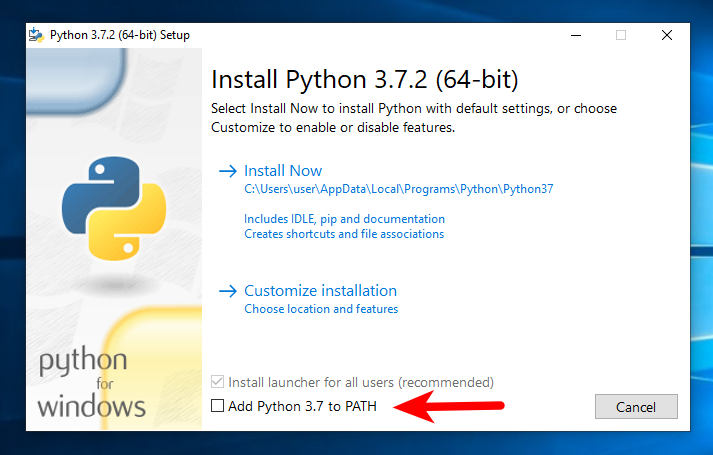
\includegraphics[width=\textwidth,height=\textheight,keepaspectratio]{python37_win_installer.png}

This box is not ticked by default, but if you don't tick it, you won't be able to type the \lstinline{python} command in a terminal, so either people tick it, add the Python installation directory manually to the system PATH, or type the full path to the Python executable.\footnote{if you choose Anaconda as a distribution, they provide a \textquote{Python console} entry in the Windows \textquote{Start} menu and their launcher to bypass this exact problem}

Adding \lstinline{python} to the system PATH works fine if you have only one Python version installed, but Windows Python executable don't have a version suffix, so if you install several Python, only one can get called from the command line: the last one added to the PATH.

To work around this, modern Python installers provide another tool on Windows, the \lstinline{py} command, which can be used just like the \lstinline{python} command (down to the same options and arguments), except you can pass a version to it: \lstinline{py -2.7} will start Python 3.7, while \lstinline{py -3.5} will start Python 3.5.

\begin{warning}
To simplify things, I will always use the \lstinline{python} command in this book. Replace it mentally with what's appropriate for you, wether it's \lstinline{python3.7} for Linux/Mac/etc or \lstinline{py -3.7} for Windows. All options and syntaxes remain the same.
\end{warning}

\section{Using a virtual environement}

As stated in the intro, the book will not explain how to use pip and virtualenv and expect you to know how.

But since you will use several Python versions, I strongly advise you to setup at least two virtual environements, one for Python 2.7, and once for Python 3.X, X depending of the version you want to port to.

I would setup two separated versions of the code, preferably using a two clones from your Version Control System (Git, Mercurial, SVN, etc) on different branches. If you don't use a VCS, now maybe a good time to learn, before starting the migration.

If you really won't use a VCS, just copy the entire code in a separate directory.

Having those 2 separate silos of code  will make things easier than having to go back and forth from one version to the other: your port may stay broken for a while during the migration, and you will probably need to fix things on the working one during that time.



\chapter{It's the little things}

As I said in the previous chapter, the big

80\% of porting your Python 2 code to Python 3 will be about little details. Thankfully, we'll see later than it can be mostly automated, so don't rush trying to change all your code base yet.


\section{Dictionaries}

To iterate on keys, values or key/value pairs, you need to use special methods in Python:

\begin{py2}
>>> population = {
...     "Octopod": 2 - 1,
...     "Xenomorph": "too many",
...     "Goa'uld": 0,
...     "Wookie": "no enough" ,
...     "Andalite": 2,
...     "Mondoshawan": "?",
... }
>>>
>>> print(population.keys())
... print(population.values())
... print(population.keys())
...
['Wookie', "Goa'uld", 'Octopod', 'Xenomorph', 'Andalite', 'Mondoshawan']
['no enough', 0, 1, 'too many', 2, '?']
['Wookie', "Goa'uld", 'Octopod', 'Xenomorph', 'Andalite', 'Mondoshawan']
\end{py2}

Because those methods produce lists, an operation that consume a lot of memory and CPU for a simple iteration, alternatives were provided.

The \lstinline{iter*} methods return a generator, sparing the need to allocate arrays:

\begin{py2}
>>> print(population.iterkeys())
... print(population.itervalues())
... print(population.iterkeys())
<dictionary-keyiterator object at 0x7f56340a0628>
<dictionary-valueiterator object at 0x7f56340a0628>
<dictionary-keyiterator object at 0x7f56340a0628>
\end{py2}

They are \gls{iterable} as well, so you can use a \lstinline{for} loop on them just like with lists, but but they can only be read once:

\begin{py2}
>>> names = population.iterkeys()
>>> list(names)
['Wookie', "Goa'uld", 'Octopod', 'Xenomorph', 'Andalite', 'Mondoshawan']
>>> list(names)
[]
\end{py2}

A better solution was found using memory views:

\begin{py2}
>>> print(population.viewitems())
... print(population.viewvalues())
... print(population.viewkeys())
dict_items([('Wookie', 'no enough'), ("Goa'uld", 0), ('Octopod', 1), ('Xenomorph', 'too many'), ('Andalite', 2), ('Mondoshawan', '?')])
dict_values(['no enough', 0, 1, 'too many', 2, '?'])
dict_keys(['Wookie', "Goa'uld", 'Octopod', 'Xenomorph', 'Andalite', 'Mondoshawan'])

\end{py2}

They save the same amount of resources, but can be read multiple times.

However, in Python 3:

\begin{itemize}
    \item \lstinline{iter*} and \lstinline{view*} methods have been removed;
    \item \lstinline{keys()}, \lstinline{values()} and \lstinline{items()} now return memory views.
\end{itemize}

So when you migrate, you want to replace all \lstinline{iter*} and \lstinline{view*} methods by regular \lstinline{keys()}, \lstinline{values()} and \lstinline{items()}. Obviously, if your code will run both in Python 2 and 3 for a while, the Python 2 code will become less performant. You can create a function to avoid this:

\begin{py2and3}
import sys

if sys.version_info.major < 3:
    def dict_items(d):
        return d.viewitems()
else:
    def dict_items(d):
        return d.items()
\end{py2and3}

And use that instead of calling the methods directly.

But don't be too hasty to do this, as in the second part of the book we will see some lirbaries that already offer those kind of tools.

One other gotcha : memory views cannot be used exactly like lists. E.G: you cannot index them (\lstinline{population.viewitems()[0]} won't work), use \lstinline{append()} on them or add them to another list.

If your code need to do that, convert them to lists before:

\begin{py3}
stats = list(population.viewitems())
\end{py3}

\section{Operations}

Coders doing a lot of maths will quickly notice de division operator has changed.

Where in Python 2 you used to do:

\begin{py2}
>>> 4 / 3
1
>>> float(4) / 3  # or you may see operator.truediv(4, 3)
1.3333333333333333
\end{py2}

In Python 3, the default division results in a float:

\begin{py3}
>>> 4 / 3
1.3333333333333333
>>> 4 // 3  # if you want the old behavior, use this new operator
\end{py3}

Now it's a trap because \lstinline{4 // 3} is valid Python 2, but it's doesn't do the same thing:

\begin{py2}
>>> 4 // 3
1
\end{py2}

Fortunatly, you can activate the behavior of Python 3 in Python 2 by adding at the top of each file:

\begin{py2and3}
from __future__ import division
\end{py2and3}

Like with \lstinline{print()}, I advise you to do this as early as possible.

Along with this change, Python 2 removed two things that I doubt you will miss but it's always good to mention.

\begin{itemize}
    \item The \lstinline{<>} operator. It was exactly like \lstinline{!=}. Just do a search and replace for this, really.
    \item The \lstinline{long} number type. When you created a big integer, Python turned it into a new type which was neither \lstinline{int} nor \lstinline{float}, and appeared suffixed with an L in the terminal (e.g: 9999999999999999999L). This is an implementation detail and you should not worry about it unless you used to parse it manually, in which case, do it in a condition.
\end{itemize}


\section{Syntax}

True = False
Exception

backtick

%https://python-future.org/compatible_idioms.html#standard-library

\section{Object oriented programming}




\chapter{Builtins}

Builtins are \glspl{callable}, mostly functions, that are available without the need for an import. E.g: \lstinline{print()} and \lstinline{len()} are builtins. They are all in the \lstinline{__builtins__} module (which is always automatically imported and available), and if you call \lstinline{dir()} on it, you'll some have been added and removed Python 3. Others are still here, but their behavior changed.

We are going to cover a lot of common and less common traps, assuming you are porting from Python 2.7 as recommanded in the introduction. Again, a lot of this can be helped with tooling, so you probably don't want to edit all your code just yet.

\section{Summary}

\begin{labeling}{summary}
\item [range() and xrange()]: \lstinline{xrange()} removed. Use \lstinline{range()}.
\item [map() and filter()]: changed behavior. Use comprehension lists.
\item [reduce()]: moved. Conditionally import from functools.
\item [input() and raw\_input()]: \lstinline{raw\_input()} removed. Alias it in V2 and use \lstinline{input()} everywhere.
\item [zip() and enumerate()]: now return generators.
\item [long()]: removed. Use \lstinline{int()}.
\item [apply()]: removed. Use unpacking.
\item [execfile()]: removed. Use \lstinline{exec(compile(open("some_module.py").read(), "some_module.py", 'exec'))}
\item [reload()]: moved. Conditionlly import it from \lstinline{importlib} and \lstinline{imp}
\item [buffer(), memoryview(), unicode() and file()]: big topic. See I/O chapter.
\item [coerce()]: deprecated. Remove.
\item [intern()]: moved. Conditionally import from \lstinline{sys}.
\item [callable()]: removed and added back. Use \lstinline{isinstance(the_thing_you_test, collections.Callable)}.
\end{labeling}

\section{range() and xrange()}

In Python 2, we had two functions, \lstinline{range()} and \lstinline{xrange()}, to generate a sequence of numbers. \lstinline{range()} produced a list, and \lstinline{xrange()} produced some kind of iterable lazy object that does the same, but without pre-computing all the values:

\begin{py2}
>>> range(3)
[0, 1, 2]
>>> for x in range(3):
...     print(x)
...
0
1
2
>>> xrange(3)
xrange(3)
>>> for x in xrange(3):
...     print(x)
...
...
0
1
2
\end{py2}

The difference is that if you do \lstinline{range(10000000000000)} and \lstinline{xrange(10000000000000)}, the first one will probably result in a \lstinline{MemoryError}, trying to fit all those numbers in RAM, while the second one will work like a charm. In any case, \lstinline{xrange()} is usually the most performant choice.

You can use a \lstinline{for} loop on both, so the added value of \lstinline{range()} was limited for the situations where you wanted to do something like slicing or using \lstinline{append()}. For this reason, \lstinline{xrange()} disapeared in Python 3, and \lstinline{range()} was set to behave like \lstinline{xrange()}.

The easy solution is to use the tools we'll talk about later to have the same \lstinline{range()} everywhere. The manual fix, however, is to replace all \lstinline{xrange()} with \lstinline{range()} and pay the performance price in Python 2 if you wish to keep the code base working with both versions. In the rare case you do need a list, convert the returned value:

\begin{py2and3}
>>> list(range(10))
[0, 1, 2, 3, 4, 5, 6, 7, 8, 9]
\end{py2and3}

\section{map() and filter()}

\lstinline{map()} and \lstinline{filter()} are simplified versions of functional programming primitives. \lstinline{map()}, in Python 2, applies a function to all elements of an \gls{iterable}, and returns a new list with the result. \lstinline{filter()} also applies a function to all elements, but returns a new list containing only the elements for which the function returned \lstinline{True}.

E.G, in Python 2:

\begin{py2}
>>> numbers = range(10)
>>> numbers
[0, 1, 2, 3, 4, 5, 6, 7, 8, 9]
>>> def is_even(num):
...     return num % 2 == 0
...
>>> filter(is_even, numbers)
[0, 2, 4, 6, 8]
>>> def power_of_2(num):
...     return num * num
>>> map(power_of_2, numbers)
[0, 1, 4, 9, 16, 25, 36, 49, 64, 81]
\end{py2}

In Python 3, they return an object that looks like a \gls{generator}:

\begin{py3}
>>> filter(is_even, numbers)
<filter object at 0x7f7b39abfa58>
>>> list(filter(is_even, numbers))
[0, 2, 4, 6, 8]
\end{py3}

This means better perfs, but unfortunalty also that you can read them only once, and you can't index them:

\begin{py3}
>>> filter(is_even, numbers)[0]
Traceback (most recent call last):
  File "<stdin>", line 1, in <module>
TypeError: 'filter' object is not subscriptable
>>> even_numbers = filter(is_even, numbers)
>>> list(even_numbers)
[0, 2, 4, 6, 8]
>>> list(even_numbers)
[]
\end{py3}

If you don't use any of the list behavior and just loop, you can let the code as-is. However, if you use any list behavior like slicing, indexing, or calling \lstinline{append()}, the you should convert the result to a list before, and store it in a variable:

\begin{py2and3}
>>> even_numbers = list(filter(is_even, numbers))
\end{py2and3}

In your code, you may also find the user of \lstinline{itertools.imap()} and \lstinline{itertools.ifilter()}. In Python 2 they were used to do the same thing as \lstinline{map()} and \lstinline{filter()}, but with the Python 3 behavior: returning generators. They've been removed, and hence, you should stick to regular \lstinline{map()} and \lstinline{filter()} only. If you are on a code base that runs on Python 2 and 3, Python 2 will have worse performances for that case.

However, idiomatic Python has a tendancy to prefer \glspl{list comprehension}, and since your are converting your code, you could take the opportunity to use them. Filtering and mapping our numbers would go from:

\begin{py2and3}
>>> list(map(power_of_2, filter(is_even, numbers)))
[0, 4, 16, 36, 64]
\end{py2and3}

To:

\begin{py2and3}
>>> [x * x for x in numbers if x % 2 == 0]
[0, 4, 16, 36, 64]
\end{py2and3}

And you can control whever you want this to produce a list or a generator by switching between \lstinline{[]} and \lstinline{()}. It solves all your problems at once: compatibility, readability and performance.

In fact, for this very particular problem, tooling will produce something less efficient than this. So embrace comprehension lists!

\section{reduce()}

\lstinline{reduce()} is another simplified functional programming primitive that helps you apply a function to two first elements of an iterable, get the result, then apply the function to the result and the next element and so on. E.g: if you wish to multiply all numbers from 1 to 10, you could do:

\begin{py2}
>>> def multiply(a, b):
...     return a * b
>>> reduce(multiply, range(1, 11))
3628800
\end{py2}

Guido Van Rossum, the creator of Python, felt like reduce was somewhat complicated to use and deserved an import. Hence, in Python 3 it is only in the \lstinline{functools} module.

There is an easy fix, as starting from Python 2.6 the function is in the builtins AND in the the \lstinline{functools} module. So all you have to do is:

\begin{py2and3}
from functools import reduce
\end{py2and3}

Once again, tooling we'll introduce later will have an automated fix for it.

\section{zip() and enumerate()}

{zip()} and enumerate() are one of those underused handy little tools. Because Python have an automatic \lstinline{for} loop and so no index incrementing, people needed another way to do things like reading two (or more) \glspl{iterable} at the same time (this is what \lstinline{zip()} does) or numbering items (which is \lstinline{enumerate()} specialty):

\begin{py2}
>>> fruits = ["Memberberries", "Gomu Gomu no Mi", "Senzus Beans"]
... is_fruit = [True, True, False]
...
>>> zip(fruits, are_fruits)
[('Memberberries', True), ('Gomu Gomu no Mi', True), ('Senzus Beans', False)]
>>> for f, status in zip(fruits, is_fruit):
...     print(f, status)
...
('Memberberries', True)
('Gomu Gomu no Mi', True)
('Senzus Beans', False)
>>> for num, f in enumerate(fruits):
...     print(num, f)
(0, 'Memberberries')
(1, 'Gomu Gomu no Mi')
(2, 'Senzus Beans')
\end{py2}

In Python 3, they do the same thing, but like \lstinline{map()} and \lstinline{filter()}, return a generator instead of a list. The coping strategy is the same as well: if you just loop once, keep it as-is, if you read it several times, index it, slice it or use list method (\lstinline{append()}, \lstinline{extend()}, etc), convert it to a list before:

\begin{py2and3}
>>> list(zip(fruits, are_fruits)) # same with enumerate()
[('Memberberries', True), ('Gomu Gomu no Mi', True), ('Senzus Beans', False)]
\end{py2and3}

In Python 2, you could find \lstinline{itertools.izip()} as an alternative to \lstinline{zip()} returning a generator. Since it doesn't exist in Python 3, always just use \lstinline{zip()}, and pay the performance penalty on Python 2 in the case you keep a Python 2/3 code base. If it's unacceptable, do a conditional import:

\begin{py2and3}
try:
    from itertools import izip
    zip = izip
except ImportError:
    pass
\end{py2and3}

And use \lstinline{zip()} everywhere as you would do for Python 3.

There is also the matter of \lstinline{itertools.izip_longest()}, a companion function to \lstinline{zip}. In case of looping on two iterables of different length, \lstinline{zip()} stops at the shortest, while \lstinline{itertools.zip_longest()} stops at the longest, filling the missing values with \lstinline{None}.

\lstinline{itertools.izip_longest()} has been renamed \lstinline{itertools.zip_longest()} in Python 3, and so you must conditionally import it:

\begin{py2and3}
try:
    from itertools import izip_longest as zip_longest
except ImportError:
    from itertools import zip_longest
\end{py2and3}

There is no such condiration for \lstinline{enumerate()}. And, of course I'm repeating myself but, we got tools for that.

\section{input() and raw\_input()}

\lstinline{input()} was seriously broken in Python 2. It's supposed to be a way to ask a question to the user and get an answer back, but what it did was to run \lstinline{eval()} on it:

\begin{py2}
>>> type(input(""))
lambda x: x
<type 'function'>
\end{py2}

This is a terrible idea security wise. So \lstinline{raw\_input()} was introduced as a way get user input, but always as a string. However, passing directly a non-ASCII string to \lstinline{raw\_input()} could trigger a \lstinline{UnicodeEncodeError}.

In Python 3, \lstinline{raw\_input()} was removed, and \lstinline{input()} just behaves like \lstinline{raw\_input()}, only it accepts transparently unicode strings.

If you migrate your code to Python 3, just replace all \lstinline{raw\_input()} with \lstinline{input()}. If you used \lstinline{input()} for it's \lstinline{eval()} capabilities, maybe it's time to avoid doing that. But if you must, just call \lstinline{eval()} manually on the result.

However, if you need to support both Python 2 and 3, you need to do something like:

\begin{py2and3}
try:
    raw\_input
except NameError: # python 3
    def eval_input(question):
        """ Use at your own risk ! """
        return eval(input(question))
else: # python 2
    eval_input = input
    input = raw\_input
\end{py2and3}

Then use \lstinline{input()} everywhere, avoid non-ASCII string in the prompt and \lstinline{eval\_input()} when you are really, really sure that's what you want to do. Or not. We will have tools for that, remember?

\section{long()}

Python 2 used to have an additional type for numbers called \lstinline{long}. Any \glspl{literal} have a way to create it with a \lstinline{callable} as well: integers can be created using \lstinline{int()}, and floats using \lstinline{float()}, so the \lstinline{long()} functions existed as well. With the type gone, the function is gone too.

If you used this function, replace it with \lstinline{int()}. Or, you know, let tools doing it for you.

\section{apply()}

\lstinline{apply()}, as the name suggests, applies a function to a list (and optionally a dict) of arguments: it's been deprecated since Python 2.3. If you used it for some reason, replace it with unpacking.

Old way that works in 2.7, but not in 3:

\begin{py2}
>>> def marvelous_function(param1, param2, like_param2_but_better):
...    print(param1)
...    print(param2)
...    print(like_param2_but_better)
...
>>> positional_params = ['First', 'Second']
>>> keyword_argument_params = {"like_param2_but_better": "Best"}
>>> apply(marvelous_function, positional_params, keyword_argument_params)
First
Second
Best
\end{py2}

New way, that works everywhere:

\begin{py2and3}
>>> marvelous_function(*positional_params, **keyword_argument_params)
First
Second
Best
\end{py2and3}

Also, tools and all that. I'm going to stop mentioning it, but you'll keep that in mind, right ?

\section{execfile()}

\lstinline{execfile("some_module.py")} is just a shorter way to do \lstinline{exec(compile(open("some_module.py").read(), "some_module.py", 'exec'))}, so use that. Although if you were doing this instead of just importing the module, there was some black magic going on, and maybe you should investigate.


\section{reload()}

When you import a module twice in Python, the job is done only once and then cached. The second time just fetches the reference from that cache: no file opening, new code parsing, no new execution. It's good for performances, and it means you can be trigger happy with the same import in many files.

But it also means if you are in the process of developping the code that if you change the file on disk and proceed to import it, nothing will happend. You need to restart the Python VM for changes to take effect.

Enter \lstinline{reload()}, a function that will allow you to reload a module without having to stop your Python program or shell. Be careful though, as it doesn't update and references, so all variables pointing to objects from this import before the reload are still holding the hold code: it can be a source of very nasty bugs, and it's why \lstinline{reload()} is not very popular.

It's also why, while it used to be a builtin in Python 2, it now needs an import. Unfortunaly, the import machinery changed between Python 3.3, where you'd have to import \lstinline{imp.reload()} and 3.4 where it's in \lstinline{importlib.reload()}. Of course, if you wish to support Python 2 and 3, you'd do:

\begin{py2and3}
try:
    from importlib import reload # 3.4+
except ImportError:
    from imp import reload # 3.3
\end{py2and3}

I insisted on tooling a few times. Ok, many times. But for this one, be careful. Some tools versions (e.g: 2to3 for Python 2) won't offer automatic transformations for this, other will, but only for \lstinline{imp.reload()} (e.g: 2to3 for Python 3.6 and lower) or \lstinline{importlib.reload()} (e.g: 2to3 for Python 3.7).

Given It's unlikely you call \lstinline{reload()} all over the place, I'd go with manual fixing on this one.

\section{buffer(), memoryview(), unicode() and file()}

Those ones need to be part of an entire chapter: the topic is notoriously misunderstood and you need to know what you're doing to have a happy migration. See \textquote{The epic tale of I/O, text and bytes}.

\section{coerce()}

\lstinline{coerce} is a relic of the past, back when Python - version 1.x ! - needed something to facilitate arythmetic operations on different types. It would take two numbers with potentially different types, and convert them to two numbers with similar values, and the same type. E.G:

\begin{py2}
>>> coerce(1, 3.)
(1.0, 3.0)
>>> coerce(1j, 3)
(1j, (3+0j))
\end{py2}

Removed in Python 3, you could emulate it with:

\begin{py2and3}
def coerce(x, y):
    t = type(x + y)
    return (t(x), t(y))
\end{py2and3}

But really, just remove it. I can't think of a single scenario using Python 2 or 3 where it would be useful. No automatic tooling will touch it, and there is no need to really: your \lstinline{DEL} key will do the job fine.


\section{intern()}

\lstinline{intern()} is a rare breed because most people have never heard of it, and never needed it, plus it's pretty low level which is exceptionnal for Python. It's used to tell Python to intern a string, keeping it in a sort of privileged cache allowing for pointer comparison. Practically, if it's used as a key in a dictionary, it will make looking it up the value faster. It the definition of a micro-optimisation, something you don't see often in this language.

In Python 3 it's been moved to \lstinline{sys.intern()}, so you can just import it, or if you need 2/3 compatible code, do a conditional import:

\begin{py2and3}
try:
    from sys import intern
except ImportError:
    pass
\end{py2and3}

But you know what they say: there are lies, damn lies and benchmarks. I've read online people can gain around 25% of perf on dict access, but my tests were closer to 5%. And again, just for one operation, dictionary look up, which is unlikely to be the bottleneck of your application. So make sure you really need it: sometimes the easiest fix is just to remove the code.

\section{callable()}

\lstinline{callable()} is a simple function returning \lstinline{True} if something is a \gls{callable}, like a function or a class. Being rarely used, it's been removed in Python 3, before being introduced again in 3.2.

If you followed the advice of not ever using Python 3.0 or 3.1, you can safely ignore this one. If you did not, you can replace it with \lstinline{isinstance(the_thing_you_test, collections.Callable)}.


\chapter{Chapter 2: imports}

Name changes, absolute imports

%https://python-future.org/compatible_idioms.html#standard-library

\chapter{All the stuff you wish you didn't have to know about I/O, text and bytes, but have to}\label{chap:text_and_bytes}

% http://www.dabeaz.com/python3io_2010/MasteringIO.pdf

Text strings in Python 3 require either 2x as much memory to store as Python 2


bad filenames were easy to create in python 2

If you ever see a \lstinline{\udcxx} character, it means that a non-decodable byte was passed in from a system interface

s.decode('utf-8','surrogateescape')

TextIOWrapper 10 times faster than codecs.open

basestring

%All backslashes in raw string literals are interpreted literally. This means that '\U' and '\u' escapes in raw strings are not treated specially. For example, r'\u20ac' is a string of 6 characters in Python 3.0, whereas in 2.6, ur'\u20ac' was the single “euro” character. (Of course, this change only affects raw string literals; the euro character is '\u20ac' in Python 3.0.)

% has been removed and reinstroduced

pathlib

%# coding: utf8

\section{file()}

\begin{py2}
from io import IOBase

if isinstance(someobj, IOBase):
\end{py2}

\section{buffer() and memoryview()}

Those two functions respectively create objects of the same name - a \lstinline{buffer} and a \lstinline{memoryview}. Both are a way to get a subset of something without copying it:

\begin{py2}
>>> donkey_lines = "Are we there yet ?\n" * 10000
>>> # this copies the data into a new object:
>>> for x in donkey_lines[:6]:
...    print(x)
A
r
e

w
e
>>> # those don't:
>>> for x in buffer(donkey_lines, 0, 5):
...    print(x)
A
r
e

w
e
>>> for x in memoryview(donkey_lines)[:5]:
...    print(x)
A
r
e

w
e
\end{py2}

It works on \lstinline{bytes}, \lstinline{bytearray}, \lstinline{array.array}...Everything that implements the so-called \textquote{buffer protocol}. This is a very nice optimization that can save quite a lot of memory/CPU if you manipulate huge chunks of bytes and pass around subset of them, e.g: to files or sockets.

With the rise of performant c libs wrapped in Python (numpy, GUI toolkits, database drivers, etc.), the need for more information about the underlying data than what \lstinline{buffer()} was offering became important. \lstinline{memoryview} provides an answer to that, being able to return the shape, dimension or type or the object behind it.

\lstinline{buffer()} is not more in Python 3, just replace it with \lstinline{memoryview()}. The later exists in Python 2.7, plus it does the same thing, just better. The only difficulty will be that \lstinline{buffer()} accepts \lstinline{unicode()} objects but \lstinline{memoryview()} only accept bytes, and so you'll need to encode them.

So:

\begin{py2}
from imaginary_lib import get_tps_reports, send_those_bytes

# Imaginary code returning a lot of bytes
tps_reports = get_tps_reports()

# Imaginary code writting those bytes to a sockets by chunks
# of 1Mio
step = 3
stop = len(tps_reports)
for i in range(0, stop, step):
    send_those_bytes(buffer(tps_reports, i, step))

\end{py2}


\chapter{Object Oriented Programming}\label{chap:oop}

\chapter{Stdlib names and behavior}

\chapter{Subtil traps}

The sys.maxint constant was removed, since there is no longer a limit to the value of integers. However, sys.maxsize can be used as an integer larger than any practical list or string index. It conforms to the implementation’s “natural” integer size and is typically the same as sys.maxint in previous releases on the same platform (assuming the same build options).

Shelve (format, ouverture)

% The from module import * syntax is only allowed at the module level, no longer inside functions.

Pickle, ssl, async/await, old style classes, .next()

\chapter{Chapter 6:  c extensions}

\part{Part 2 : how to migrate}

\chapter{Chapter 5 : how NOT to migrate}

Pypy, nuikta, docker, vendoring, pex, pinpoint dependancies

\chapter{Chapter 5 bis: prepare your project}

Get rid of *.

Get rid of old style class.

Write test if you can. Pytest.

Setup linters and text formatter.

Decide if you want a compatible code base or a migration

Can you use mypy ?

Don't do anything else while migrating.

Stop all python 2 new project.

\chapter{Chapter 6: low hanging fruits}

2 to 3, from future, manuall fixing

(Still using 2.6:) Turn on the -3 command line switch. This enables warnings about features that will be removed (or change) in 3.0. Run your test suite again, and fix code that you get warnings about until there are no warnings left, and all your tests still pass.

\chapter{Chapter 7 : Chapter restructuring the project}

Imports, layout,

\chapter{Chapter 7: compatible code base}

Python future, backports

\chapter{Chapter 8: fighting deprecation}

What to replace with what ?

\chapter{Chapter 9 : bytes and str}

Pathlib, open, network, u, future...

\chapter{New features to take advantage of}\label{chap:new_features}

%print()

Fstring

Asyncio

Statistic

Debug

Dataclass

\appendix

\printglossaries

\backmatter %bibliography


When Python 2 End of Line was announced, the step by step migration guide the community followed looked a lot like:

\begin{enumerate}
\item Denial
\item Anger
\item Bargaining
\item Depression
\item Acceptance
\end{enumerate}

This book is about all the steps after that. We'll supposed you decided what to do now, and we will provide you with the help to do it:

\begin{itemize}
\item Some advices on which Python versions to choose, the one to port from, and the one to port to. Or not port to.

\item An in depth description of the differences between Python 2 and 3. And since we know the code you work on may not be your own, it will come with details on what all this stuff does, why it changed, and what are the consequences.

\item Solutions to stay on Python 2 for the decade to come. Yes, it's possible. Nobody told you ?

\item A migration strategy to either  move your project to something that works in Python 2 and 3, or just Python 3. Or both.

\item Tooling to support and even automatize the process as much as we can. Because we are coders after all.

\item And along the way, some nice, long and cristal clear explanations on complicated topics like encoding or object oriented programming.
\end{itemize}

In fact, weither you migrate your code or not, you'll be a better Python programmer after reading this book.


\end{document}
